\documentclass{article}

\usepackage{amsmath,amssymb,amsthm,fancyhdr}
\usepackage[margin = 1.5in]{geometry}
\usepackage{graphicx}
\usepackage{url}
\usepackage{upquote}
%\setlength{\parindent}{0pt}

\pagestyle{fancyplain}

%\chead{\LARGE{Math stuff}}
%\rhead{Summer 2022}

\newcommand{\C}{{\mathbb C}}
\newcommand{\F}{{\mathbb F}}
\newcommand{\N}{{\mathbb N}}
\newcommand{\Q}{{\mathbb Q}}
\newcommand{\R}{{\mathbb R}}
\newcommand{\Z}{{\mathbb Z}}

\begin{document}

\iftrue
\begin{titlepage}
    \begin{center}
        \vspace*{1cm}
            
        \Huge
        \textbf{Visualizing the Intersection between a Cubic Surface and a Plane}
            
        \vspace{0.5cm}
        \LARGE
            
        \vspace{1.5cm}
            
        \text{Isabella Harker}
        
        \vspace{1.5cm}
        
        \large

            
        \vfill  
            
        \vspace{0.8cm}
            
        \Large
        Department of Mathematics\\
        University of Oregon\\
        September 2022
            
    \end{center}
\end{titlepage}
\fi

\section*{Introduction}
   
	
	A curious fact about smooth cubic surfaces is that they all contain exactly 27 straight lines, although some of those lines may be complex or exist only at infinity. Considering a cubic surface in $\R^3$, there will be a variable number of straight lines contained in the surface, although at least one straight line is real for every cubic surface. We can find all 27 lines by projectivizing the surface in $\C P^3$ for a cubic surface of dimension 2, which allows us to consider both the complex straight lines and the lines `at infinity' \cite{lines}. However, it is also possible to choose a surface containing only real lines, which the surface in the video is an example of, and choosing such a surface makes visualizing the surface easier.
	
	Given a straight line $L$ contained in a cubic surface and taking the set of all planes which also contain $L$, the intersection between any plane in that set and the cubic surface will be a conic, plus $L$. Furthermore, there are exactly 5 planes where the conic degenerates to two lines, although they can be either complex or at infinity, so it is not always possible to visualize all 5 planes. Analytically, this is because when a substitution is made to find the equation of the conic, we find a 3rd-degree polynomial which contains a straight line, so a linear factor can be factored out of the polynomial, leaving a conic. 

	Section 1 demonstrates this concept analytically using Fermat's cubic surface, by first finding a line and planes then showing the factorization of the conic. Section 2 then explains our analysis of the cubic surface shown in the videos, and Section 3 describes the process of rendering the videos. \\
	
	This work was supported by NSF grant no. DMS-2039316.

\iftrue
\newpage
\section{Fermat's Cubic surface}
	%render better image of Fermat's Cubic surface
	\begin{figure}[h!]
		\centering
		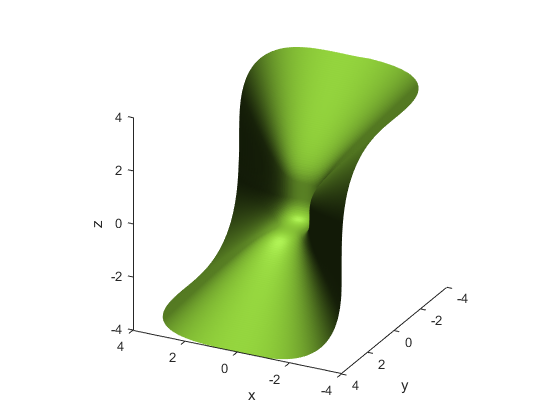
\includegraphics[scale=0.75]{fermat_cubic_image.png}
		\caption{Fermat's Cubic surface}
		\label{fermat_fig}
	\end{figure}
	We begin by examining Fermat's cubic surface,
	\[ x^3 + y^3 + z^3 + 1 = 0, \]
	which contains the real line 
	\[x + 1 = 0, y + z = 0 \]
	for all $x, y, z \in \R$. This line can also be parametized as 
	\[ \langle1, t, -t \rangle, t \in \R \]
	Denote the above line $L_f$. Now that we have found a line, the second step is to find the set of planes which also contain $L_f$. Starting with the general equation for a plane, 
	\[ ax + by + cz + d = 0, \]
	we find that all points $(-1, t, -t), t \in \R$ are contained in the plane when the equations
	\[ -a + d = 0 \]
	\[ b - c = 0 \]
	are both satisfied. So, we conclude that the set of all planes which contain $L_f$ is 
	\[ \{ x + ay + az + 1 = 0, y + z = 0 : a \in \R \} \]
	
	The first method to find the intersection of the plane and the cubic surface would be to solve for $z$, which is useful if we want to visualize the curve of intersection in 3D-space. This is the method used to produce the videos. However, if we want to be able to visualize a projection of the curve in 2D, it is better to parametize the curve using vectors which lie in the plane, preferably orthogonal vectors. This second method is explained below.
	
	For a plane with the general equation 
	\[ x + ay + az + 1 = 0, \]
	we can take the three points on the plane
	\[ (-1, 0, 0), (-1, 1, -1), (0, 1, -a-1) \]
	and find two vectors 
	\[ u_1 = \begin{bmatrix} 0 \\ 1 \\ -1 \end{bmatrix}, u_2 = \begin{bmatrix} 1 \\ 1 \\ -a-1 \end{bmatrix} \]
	Orthogonalizing this pair of vectors gives us the set 
	\[ v_1 = \begin{bmatrix} 0 \\ 1 \\ -1 \end{bmatrix}, v_2 = \begin{bmatrix} 1 \\  - \frac{a}{2} \\ -\frac{a}{2} \end{bmatrix} \]
	Using these two vectors to parametize the plane by writing each variable $x,y,z$ as $u\cdot v_1 + v\cdot v_2$ for some $u, v$ and including the displacement of $(-1, 0, 0)$, we have 
	\begin{align*}
	x &= v - 1\\
	y &= u - \frac{a}{2} v\\
	z &= -u - \frac{a}{2} v \end{align*}
	
	We can use this parametization to find an equation for the intersection between the plane and the surface by substituting these parametizations into the equation for the surface. This gives us
	\[ \left(v-1 \right)^3 + \left(u - \frac{a}{2}v \right)^3 + \left(-u - \frac{a}{2} v \right)^3 + 1 = 0, \]
	which can be expanded and simplified to 
	\[ v\left( \left(1-\frac{a^3}{4} \right)v^2 - 3au^2 - 3v + 3 \right) = 0 \]
	This equation shows the two parts of the intersection. The line $v = 0$ is the same line that is contained in the surface, that is, 
	\[ x + 1 = 0, y + z = 0, \]
	and the other factor in the product is an elliptic curve, which shows that the intersection between the cubic surface and a plane containing the given line consists of an elliptic curve and the line. The substitution shown above can also be graphed for different values of $a$, which gives a visual representation of the intersection. This conic is usually an ellipse or hyperbola, however there are some points where the intersection is a pair of lines. In this case, the intersection is a pair of lines for the value $a = 1$. 
	
	Substituting linear values for $x,y,z$ yields a cubic polynomial from which the starting line can always be factored. Once the line is removed, the polynomial which remains forms a one-parameter family of conics in two variables, where the parameter defines the plane of intersection. 
	
	It is possible to repeat the process shown above for Fermat's cubic surface with any cubic surface, however, the lines contained within the surface are frequently more complicated than the above line, as the following cubic surface demonstrates. As a result, it is typically easier to avoid parametization altogether and instead work with the original variables $x, y, z$. This is how we made the videos, both because of this complexity and because we wanted to visualize the intersection in 3 dimensions. 
\fi
	
\newpage
\section{KM1}
	
		The cubic surface shown below and in the videos represents one topological type of real projective cubic surfaces as classified by Kn{\H o}rrer and Miller. For this particular type, all 27 lines contained within the surface are real, making it a good tool for visualization since all of these lines can be graphed in $\R^3$.
	
	The equation of the cubic surface is 
	\[ f(x,y,z) = 4x^3-12xy^2+3x^2z+3y^2z-\frac{17}{2}z^3-\frac{9}{2}x^2-\frac{9}{2}y^2-12z^2-3z+2 \label{km1_eqn}, \]
	evaluated at $f(x,y,z) = 0$, which produces the graph shown below \cite{km_surf}.
	
	\begin{figure}[h!]
		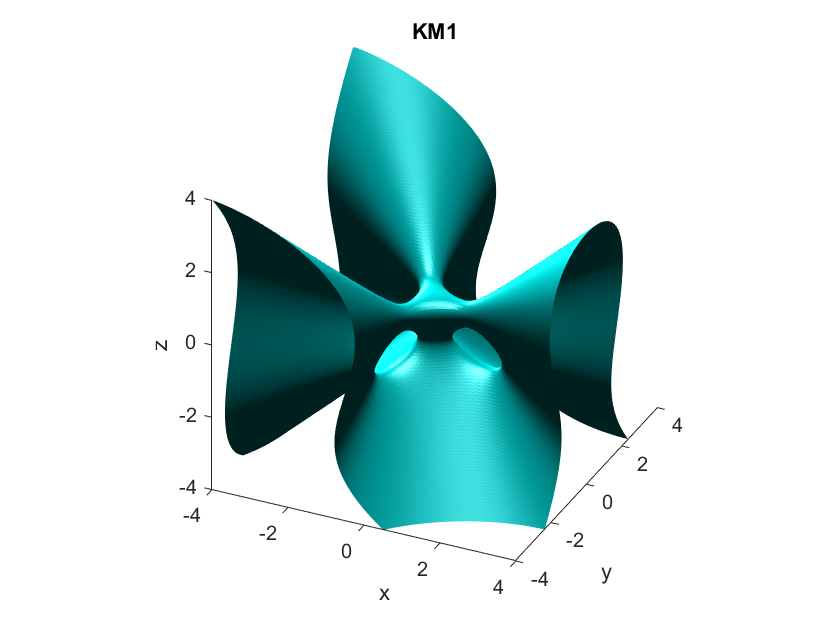
\includegraphics[scale=0.50]{km1_img.png}
		\centering
		%\caption{etc}
		\label{km1_fig}
	\end{figure}
	
	
	
	It turns out that one of the lines contained in $f(x,y,z)$ is the line 
	\[ L_k = \langle x_1, t, z_1 \rangle, \label{km1_line} \]
	where $z_1$ is the biggest root of $264 z^3 + 420 z^2 + 42 z - 37$ and $x_ 1 = \frac{z_1}{4} - \frac{3}{8}$, or,
	\[ z_1 = \frac{-35  + \frac{944}{\sqrt[3]{-10601 + 33i \sqrt{798647}}} + \sqrt[3]{-10601 + 33i \sqrt{798647}}}{66} \approx 0.236792032999024 \]
	\[ x_1 = \frac{z_1}{4} - \frac{3}{8} \approx -0.315801991750244 \]
	%FIXME ???????????
	% ``it turns out ``
	%nick found the line
	
	The set of all planes containing $L_k$ is all those for which
	\[ \{ a(x-x_1) + b(z-z_1) = 0: a, b \in \R \} \]
	For the sake of computational simplicity, this can be rescaled to have only one parameter, although plane where the second parameter is equal to 0 must also be included. After scaling, we have 
	\[ \{ (x,y,z): a(x-x_1) + z-z_1 = 0,  a \in \R \text{ or } x - x_1 = 0 \} \]
	On this particular surface, the plane $x-x_1 = 0$ is not one where the conic is degenerate, therefore we don't need to consider it in our calculations, however this may not be the case for all cubic surfaces. In fact, if we scaled the planes based on $x$ instead of $z$, we would have to consider the plane $z-z_1 = 0$, since the conic is degenerate at that point. 
	
	Instead of parametizing the variables using vectors contained in the plane, we are going to continue using $x,y,z$. The next step is to find the general equation for the conic in terms of $a$, which is done by substituting
	\[ z = z_1 - a(x-x_1) \]
	into the equation for the cubic surface, then factoring the line $x-x_1$ from the resulting cubic. What remains is a conic in $x$ and $y$, 
	\begin{equation}
	\begin{aligned}
	&\left(3a-\tfrac{17}{2}a^3-4 \right)x^2 +\left(3a+12 \right)y^2+\left(17a^3 x_1 +12a^2-4x_1 -3z_1-\tfrac{9}{2} +\tfrac{51}{2}a^2z_1 \right)x \\ 
	&-\tfrac{17}{2}a\left(3z_1^2+3az_1x_1-a^2x_1^2 \right)-12a\left(2z_1+ax_1 \right)-3a-4x_1^2-\left(4z_1-\tfrac{9}{2} \right)x_1 = 0 \label{conic_eqn}
	\end{aligned}
	\end{equation}
	
	Now that we have a set of elliptic curves in $x,y$, all that remains is to find the values of $a$ for which the curve is degenerate. From \textit{On Degenerate Conics} by J.W.Lasley, Jr., given some conic 
	\[ ax^2 + 2hxy + by^2 + 2gx + 2fy + c = 0, \]
	it is degenerate if and only if the matrix
	\[ \begin{bmatrix} a & h & g \\ h & b & f \\ g & f & c \end{bmatrix} \]
	has determinant equal to 
	0 \cite{10.2307/2309606}. Applying this to our conic ($\ref{conic_eqn}$), we find that the planes $a(x-x_1) + z-z_1 = 0$ for which the intersection becomes a trio of lines is precisely those where $a$ is a root of the 5th-degree polynomial
	\begin{multline*}
	\left( 3a-12 \right) \big( \left( \tfrac{1683}{32}z_1^2+\tfrac{1785}{32}z_1-\tfrac{1803}{128}  \right) a^4+ \left( -\tfrac{603}{16}z_1+\tfrac{1809}{32} \right) a^3\\
	+ \left(-\tfrac{603}{4}z_1-63 \right)a^2+ \left(99z_1^2+105z_1+\tfrac{21}{4} \right) a \big) = 0, 
	\end{multline*}
	
	which are the values
	\[ \{ -24.92066225, -4, 0, 0.47015845, 1.469357367 \}, \]
	so the planes for which the conic is degenerate happen at the 5 points in time above. 
	
	In the videos, the equation for the plane is shown at the top, and the numbers don't match the values of the roots. This is due to the parametization of the plane as
	\[ \left( \cos \theta \right) x + \left( \sin \theta \right) z = \left( \cos \theta \right) x_1 + \left( \sin \theta \right) z_1 \]
	as $\theta$ varies constantly with time, which ensures that the plane rotates at a constant angular speed around the line $L_k$. This parametization is practically equivalent to normalizing the plane equation, $a(x-x_1) + z-z_1 = 0$, so the planes with degenerate conics were found by taking $\cot \theta$ to be equal to the values of the 5 roots. 

	\newpage
	\section{Graphing}
	I used Matlab to create the videos, following the method described in \cite{isosurface}.
	
	Starting with the equation for KM1 as described above and the set of planes containing the line $L$, I used the isosurface function to create a 3D mesh of the surface.
	\iffalse
	\begin{figure}[h!]
		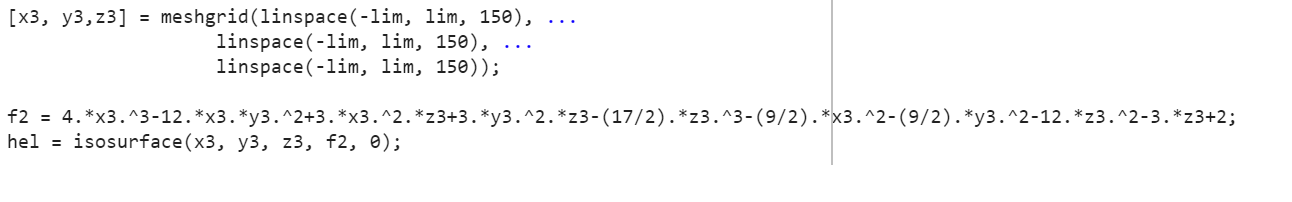
\includegraphics[scale=0.75]{km1_function.png}
		%\caption{Code to generate KM1}
		\label{km1_eqn_fig}
	\end{figure}
	\fi
	
	\begin{verbatim}
    [x3, y3,z3] = meshgrid(linspace(-lim, lim, 150), ...
                   linspace(-lim, lim, 150), ...
                   linspace(-lim, lim, 150));

    f2 = 4.*x3.^3-12.*x3.*y3.^2+3.*x3.^2.*z3+3.*y3.^2.*z3-(17/2).*z3.^3-(9/2).*x3.^2 -   
     (9/2).*y3.^2-12.*z3.^2-3.*z3+2;
    hel = isosurface(x3, y3, z3, f2, 0);
\end{verbatim}
	
	The isosurface function creates a surface made up of triangular faces, so the intersection consists of all faces which have 1-2 vertices above some plane $P$.
	
	\iffalse
	\begin{figure}[h!]
		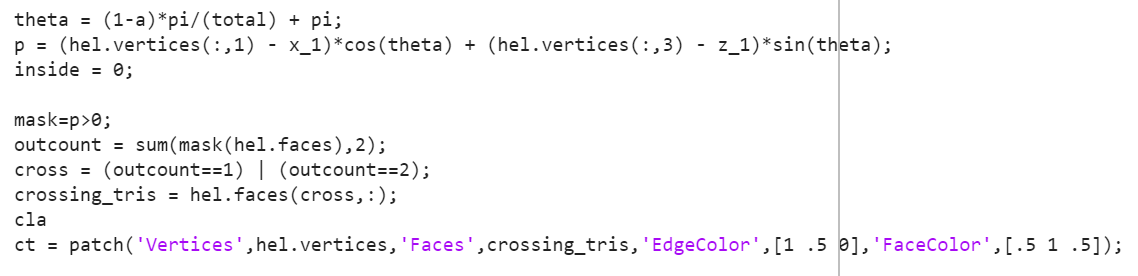
\includegraphics[scale=0.75]{km1_plane_intersect.png}
		%\caption{Creating a logical mask using the equation of the plane}
		\label{km1_intersect_fig}
	\end{figure}
	\fi
	
	\begin{verbatim}
    theta = (1-a)*pi/(total) + pi;
    p = (hel.vertices(:,1) - x_1)*cos(theta) + (hel.vertices(:,3) - z_1)*sin(theta);
    inside = 0;
    
    mask=p>0;
    outcount = sum(mask(hel.faces),2);
    cross = (outcount==1) | (outcount==2);
    crossing_tris = hel.faces(cross,:);
    \end{verbatim}
	Using a logical mask, I was able to isolate the part of the surface which intersects $P$, then use only that set of faces to generate the line of intersection. 
	
	\iffalse
	\begin{figure}[h!]
		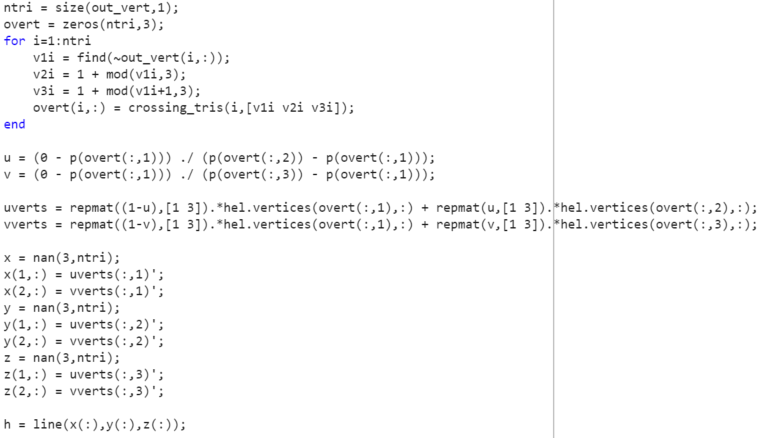
\includegraphics[scale=0.75]{intersect_line.png}
		%\caption{etc}
		\label{km1_intersect_line_fig}
	\end{figure}
	\fi
	
	\begin{verbatim}
	    ntri = size(out_vert,1);
    overt = zeros(ntri,3);
    for i=1:ntri
        v1i = find(~out_vert(i,:));
        v2i = 1 + mod(v1i,3);
        v3i = 1 + mod(v1i+1,3);
        overt(i,:) = crossing_tris(i,[v1i v2i v3i]);
    end
    
    u = (0 - p(overt(:,1))) ./ (p(overt(:,2)) - p(overt(:,1)));
    v = (0 - p(overt(:,1))) ./ (p(overt(:,3)) - p(overt(:,1)));
    
    uverts = repmat((1-u),[1 3]).*hel.vertices(overt(:,1),:) + 
    repmat(u,[1 3]).*hel.vertices(overt(:,2),:);
    vverts = repmat((1-v),[1 3]).*hel.vertices(overt(:,1),:) + 
    repmat(v,[1 3]).*hel.vertices(overt(:,3),:);
    
    x = nan(3,ntri);
    x(1,:) = uverts(:,1)';
    x(2,:) = vverts(:,1)';
    y = nan(3,ntri);
    y(1,:) = uverts(:,2)';
    y(2,:) = vverts(:,2)';
    z = nan(3,ntri);
    z(1,:) = uverts(:,3)';
    z(2,:) = vverts(:,3)';
    
    h = line(x(:),y(:),z(:));
    \end{verbatim}
    
	Once I found the correct set of faces, I smoothed the line of intersection by turning each triangular face into a single vertex of the line. Finally, I joined all the vertices into a single line object at the end, which I then graphed. This method can be used for any two surfaces, since it relies only on the equations of the surfaces themselves, and furthermore it isn't necessary to know the equation of the line of intersection, since the line is created from the intersection at a software level based on the values of the functions at each vertex.
	
	\iffalse
	\begin{figure}[h!]
		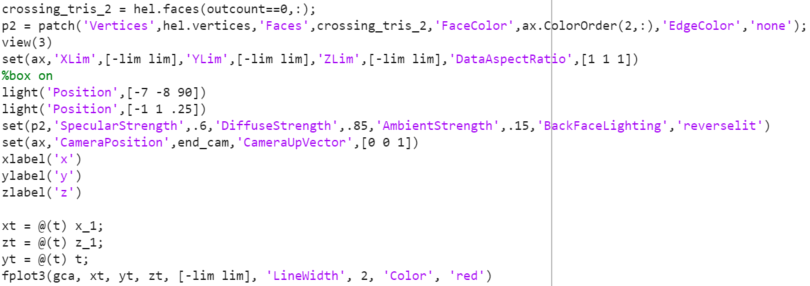
\includegraphics[scale=0.75]{final_image_km1.png}
		%\caption{etc}
		\label{km1_final_code_fig}
	\end{figure}
	\fi
	
	\begin{verbatim}
	    h.Color = ax.ColorOrder(5,:);
    h.LineWidth = 2;

    crossing_tris_2 = hel.faces(outcount==0,:);
    p2 = patch('Vertices',hel.vertices,'Faces',crossing_tris_2
    ,'FaceColor',ax.ColorOrder(2,:),'EdgeColor','none');
    view(3)
    set(ax,'XLim',[-lim lim],'YLim',[-lim lim],'ZLim',[-lim lim],'DataAspectRatio',[1 1 1])
    light('Position',[-7 -8 90])
    light('Position',[-1 1 .25])
    set(p2,'SpecularStrength',.6,'DiffuseStrength',.85,
    'AmbientStrength',.15,'BackFaceLighting','reverselit')
    set(ax,'CameraPosition',end_cam,'CameraUpVector',[0 0 1])
    xlabel('x')
    ylabel('y')
    zlabel('z')

    box off

    hold on

    xt = @(t) x_1;
    zt = @(t) z_1;
    yt = @(t) t;
    fplot3(gca, xt, yt, zt, [-lim lim], 'LineWidth', 2, 'Color', 'red')
    \end{verbatim}
	The final step is to graph the line along with the portion of the surface which lies below the plane, which can be done using the same logical mask that I initially used to find the line of intersection. This clearly shows that as the plane rotates around the line $L_k$, the intersection is always a conic. Furthermore, it is degenerate at 5 points in time. 
	
	\newpage
	\begin{figure}[h!]
		\centering
		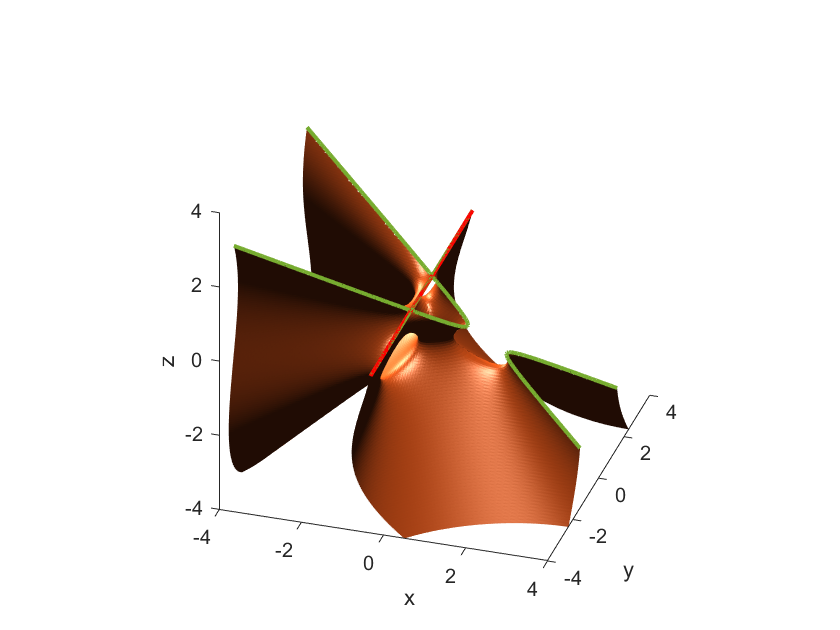
\includegraphics[scale=0.50]{graphing_end_result.png}
		%\caption{etc}
		\label{km1_final_fig}
	\end{figure}

	After all the steps are taken, the final image looks like the one shown above.
	
	While it is not always completely clear from the video that the intersection is a conic, this is because the software cannot use exact values for every plane, so some of the degenerate planes are not exact. The analytical solution gives the exact equation for these 5 planes. 
	
	The videos consist of two images side-by-side, one showing the line of intersection and the other showing the plane and the surface. This method was chosen to aid in visualizing both the conic and the plane that creates the conic. To make the videos, we rendered successive frames as the plane slowly rotated, and in one video paused at all of the planes where the conic is degenerate. 
	
\newpage

\addcontentsline{toc}{section}{References}
\nocite{*}
\bibliographystyle{ieeetr}
\bibliography{int_cit}



\end{document}